\documentclass[a4paper]{article}
\PassOptionsToClass{final}{article}
\usepackage[final]{graphicx} % Required for inserting images
\usepackage{fontspec} % For English display
\usepackage{xeCJK} % For Chinese & Japanese display
\usepackage{multicol}
\usepackage{tikz}
\usepackage{xcolor}
\usepackage{xparse}
\usepackage{subcaption}
\usepackage{tabularx}
\usepackage{eso-pic}
\usepackage{contour}
\contourlength{1pt} % 轮廓粗细
\usepackage[
    colorlinks=true,
    linkcolor=blue,
    urlcolor=blue,
    citecolor=blue
]{hyperref}
\usepackage{geometry}
% BE CAREFULE: IF YOU WANT TO ADD CHINSES, DO NOT EDIT THIS FILE
% GO TO Chinese.tex

\setlength{\parindent}{0pt}

%%%%%%%%%%%%%%%%%%%%%%%%%%%%%%%%%%%%%%%%%%%%%%%%%%%%%%%%%%%%%%%
% File structure
%
% Root
%root/
%├── Figs/                            You should put all figures here
%│
%├── Alice.ttf                        ttf file for the dwarf language
%│
%├── Alice.kbitx                      design file for dwarf language
%│
%├── BitsNPicas.jar                   Program to edit Alice.kbits
%│
%├── Japanese.tex                     Japanese tex file
%└── Chinese.tex                      Chinese tex file
%%%%%%%%%%%%%%%%%%%%%%%%%%%%%%%%%%%%%%%%%%%%%%%%%%%%%%%%%%%%%%%

\definecolor{mygreen}{RGB}{30,90,55}
\definecolor{myorange}{RGB}{234,102,44}
\definecolor{myred}{RGB}{170,0,41}

%%%%%%%%%%%%%%%%%%%%%%%%%%%%%%%%%%%%%%%%%%%%%%%%%%%%%%%%%%%%%%%
% Set some fonts for display
% I chosen them based on my taste, feel free change them if needed
% These are supported fonts:
% https://www.overleaf.com/learn/latex/Questions/Which_OTF_or_TTF_fonts_are_supported_via_fontspec%3F#!CJK
%%%%%%%%%%%%%%%%%%%%%%%%%%%%%%%%%%%%%%%%%%%%%%%%%%%%%%%%%%%%%%%
\setmainfont{x12y16pxMaruMonica.ttf} % Eng display
\newCJKfontfamily\zhfont{HYPixel11pxU-2.ttf} % 中文
\newCJKfontfamily\jpfont{x12y16pxMaruMonica.ttf} % 日文
\newfontfamily\PUAfont{Alice.ttf}[
  Range = {U+0100-U+017F}
]

%%%%%%%%%%%%%%%%%%%%%%%%%%%%%%%%%%%%%%%%%%%%%%%%%%%%%%%%%%%%%%%
% Paper length & width
%%%%%%%%%%%%%%%%%%%%%%%%%%%%%%%%%%%%%%%%%%%%%%%%%%%%%%%%%%%%%%%

\newgeometry{margin=0cm}
\begin{document}
% \title{\jpfont{\Huge {Alice In Cradle} 0.29 WPE Dwarf Language Interpretation result\\ \textit{Alice In Cradle} 0.29 WPE ドワーフ 語 解読結果}}
\null
\AddToShipoutPictureFG*{%
  \put(0.5\paperwidth,0.7\paperheight){%
    \makebox(0,0){%
      \begin{minipage}{0.8\paperwidth}
        \centering
        {\bfseries\scalebox{2}{\contour{black}{\textcolor{white}{{Alice In Cradle} 0.29 WPE Dwarf Language Interpretation result}}}\\[2em]{\bfseries\scalebox{2.5}{
          \contour{black}{\textcolor{white}{\jpfont{Alice In Cradle 0.29 WPE ドワーフ 語 解読結果}}}}}\\
        }
      \end{minipage}
    }
  }
}



\AddToShipoutPictureBG*{%
  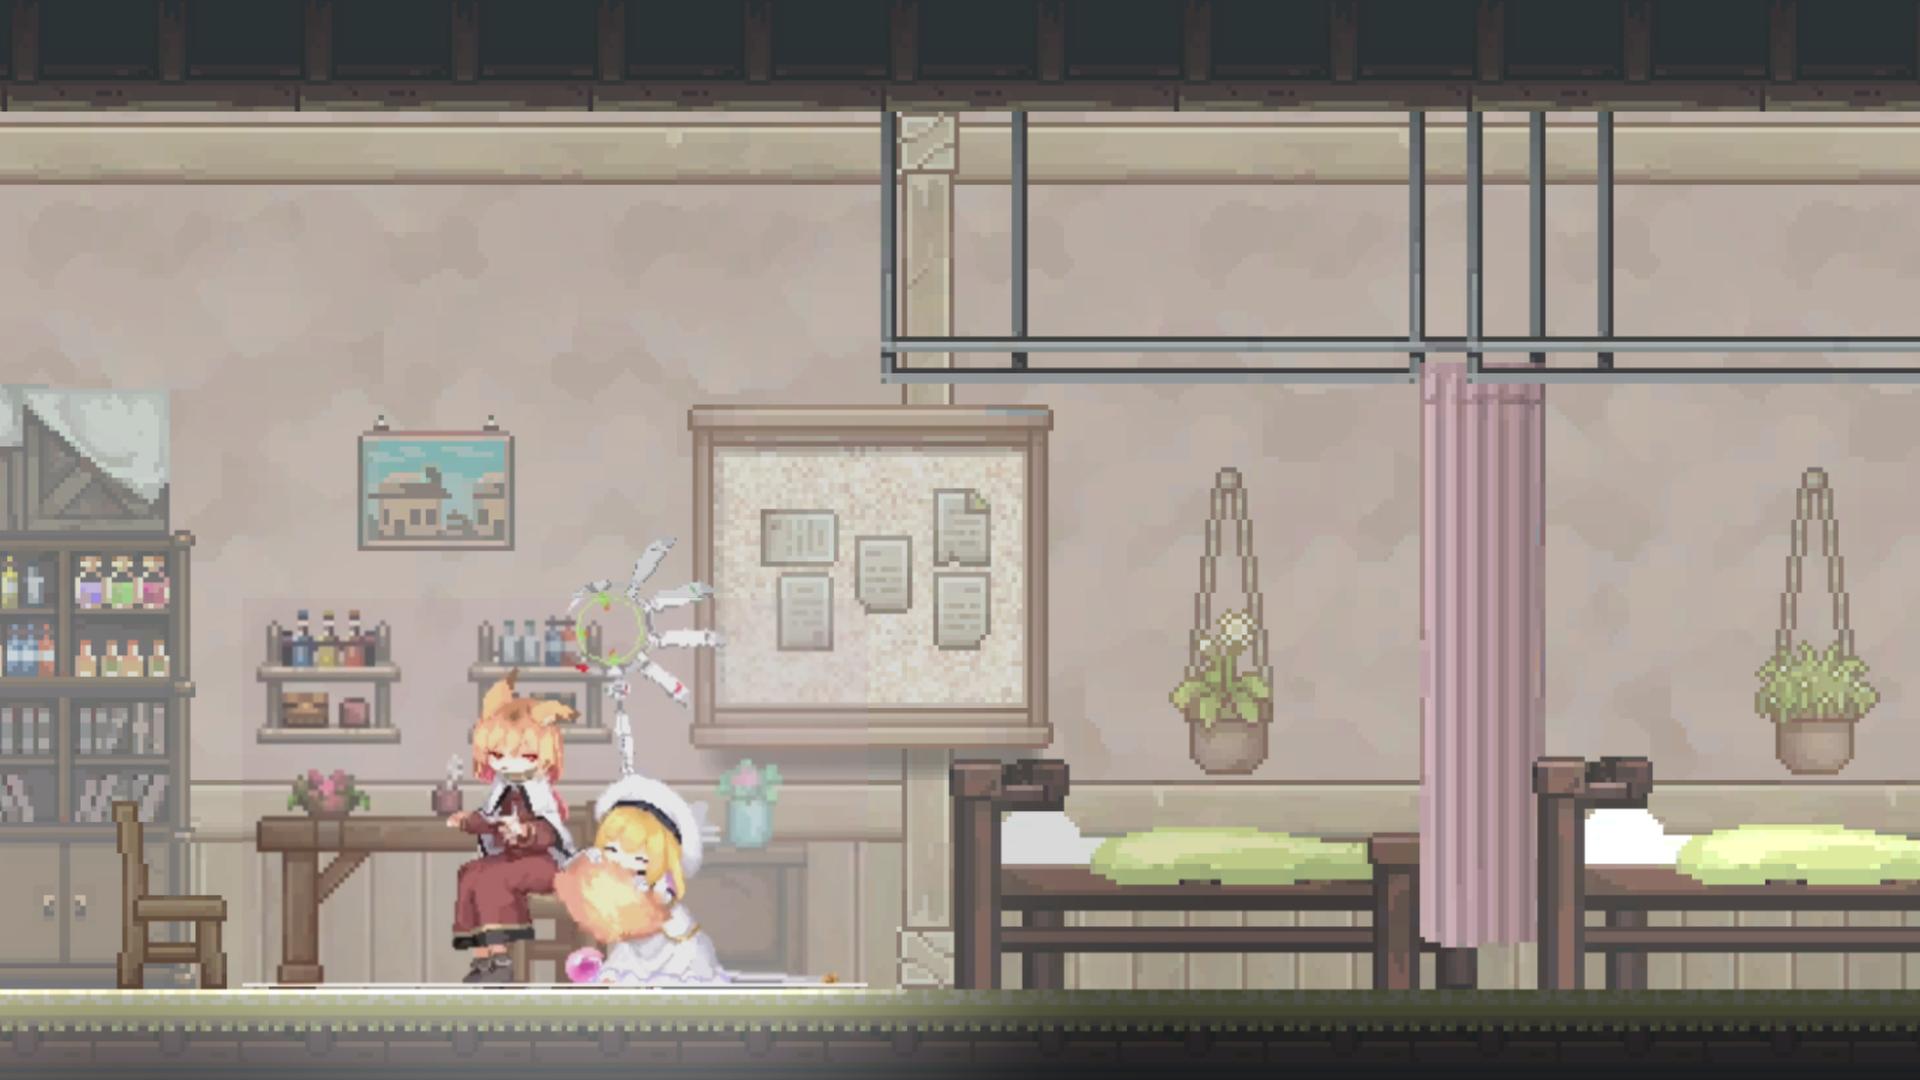
\includegraphics[height=\paperheight]{Figs/Others/mofu.png}
}

\thispagestyle{empty}
\clearpage

\newgeometry{
  a4paper,          
  left=1cm,
  right=1cm,
  top=1cm,
  bottom=1cm
}

\AddToShipoutPictureBG{%
  \AtPageLowerLeft{%
    \includegraphics[width=\paperwidth,height=\paperheight]{Figs/Others/frame.png}%
  }%
}
\textbf{\jpfont{すべての英語コンテンツには日本語訳が付いています。}}
\section{Introduction / \normalfont{\jpfont{前置き}}}
\subsection{Credibility / \normalfont{\jpfont{信頼性}}}
We use colors to represent the credibility of the translation:\\
{\color{mygreen}Green}: The result is 100\% correct.(Unless their meaning changed in further versions).\\
{\color{myorange}Orange}: We are confident in the result, but we can't promise they are correct.\\
{\color{myred}Red}: We are not confident in the result, in other words, they are basically random guessing.\\\\
Most translations are in {\color{myorange}orange state}, because we will only set translation to {\color{mygreen}green state} when we have very strong evidence to prove the credibility(which will be introduced later).\\\\
Also, sometimes it is too difficult to translate some sentences, since most of their words appeared only once. Under that circumstance, we would use "({\color{myred}[We are unable to translate this]})({\color{myred}\jpfont{[合理的な翻訳は得られない]}})" to mark them. Luckily, most sentences are translatable.\\\\
\jpfont{翻訳の信頼性を表すために色を使用しています:}\\
\jpfont{{\color{mygreen}緑色: }結果は100\%正確だ。}\\
\jpfont{{\color{myorange}オレンジ: }結果には自信がありますが、それが正しいとは保証できません。}\\
\jpfont{{\color{myred}赤色: }結果には自信がありません。言い換えれば、推測だけです。}\\\\
\jpfont{ほとんどの翻訳は{\color{myorange}オレンジ状態}です。これは、信頼性を証明する非常に強力な証拠がある場合にのみ、翻訳を{\color{mygreen}緑色状態}に設定するためです(証拠は後で紹介されます)。}\\\\
\jpfont{また、文を構成するシンボルに一度しか登場しないシンボルの数が多いすぎる場合では、翻訳ができない場合もあります。その時、"({\color{myred}[We are unable to translate this]})({\color{myred}\jpfont{[合理的な翻訳は得られない]}})"を使ってマークします。幸いなことに、翻訳できないの比例は少ないです。}

\subsection{References / \normalfont{\jpfont{参考資料}}}
In addition to ordinary materials like stream video, we have also got some very powerful hint by unpacking the game. \\\\
As shown in the figure (a) , we have found this picture from one released game version. Many symbols occurred in this manuscript are also used in the preview version, so this picture is basically a "Trust Anchor" for our translation.\\
As shown in figure (b), we are able to call some dwarf symbols and their pronunciation in 0.28i version. We have developed a hypothesis based on it: Most dwarf words pronounce the leading syllable of it's Japanese translation. For example, {\PUAfont \symbol{"0120}}, whose meaning is "You", reads as "Ki", and the pronunciation of "You" in Japanese is "Ki Mi".\\\\
\jpfont{配信ビデオで得た資料に加えて、ゲームをデシリアライゼーションすることによって、役に立つ情報も得ました。}\\\\
\jpfont{図(a)に示すように、あるAICバージョンからこの原稿を発見しました。この原稿に登場する多くの記号はセリフでも使用されているため、この原稿は基本的に私たちの翻訳の「信頼アンカー」と言えます。}\\
\jpfont{図(b)に示すように、バージョン0.28iで一部の「dwarf語」シンボルとその日本語の発音を呼び出せました。私たちはこの情報に基づいて仮説を立てました。ほとんどの「dwarf語」シンボルは日本語訳の先頭の音節を発音します。例えば、{\PUAfont \symbol{"0120}}の意味は”きみ”、そしてその発音は”き”。}

\begin{figure}[htbp]
\begin{subfigure}{0.45\textwidth}
    \centering
  \includegraphics[height=6cm]{Figs/Others/character_dwarf.png}
  \caption{Hashino's manuscript / \jpfont{はーちゃんの原稿}}
\end{subfigure}
\begin{subfigure}{0.45\textwidth}
  \centering
  \includegraphics[height=6cm]{Figs/Others/loaded_4_3.png}
  \caption{Japanese pronunciation of some symbols / \jpfont{いくつかのシンボルの発音}}
\end{subfigure}

\end{figure}


\newpage
%%%%%%%%%%%%%%%%%%%%%%%%%%%%%%%%%%%%%%%%%%%%%%%%%%%%%%%%%%%%%%%
% In this section, you should write:
% 1. A table showing all discovered symbols
%%%%%%%%%%%%%%%%%%%%%%%%%%%%%%%%%%%%%%%%%%%%%%%%%%%%%%%%%%%%%%%
\section{All discovered dwarf symbols / \normalfont{\jpfont{発見したシンボル}}}
%%%%%%%%%%%%%%%%%%%%%%%%%%%%%%%%%%%%%%%%%%%%%%%%%%%%%%%%%%%%%%%
% Table showing all alice-language words and their translations
%%%%%%%%%%%%%%%%%%%%%%%%%%%%%%%%%%%%%%%%%%%%%%%%%%%%%%%%%%%%%%%
\begin{table}[htbp]
  \Large
  \begin{minipage}[t]{0.15\textwidth}
    \vspace{0pt}
    \centering
    \begin{tabular}{ll}
        \hline
        Symbols & code \\
        \hline
        {\PUAfont \symbol{"0100}} & 0100\\
        {\PUAfont \symbol{"0101}} & 0101\\
        {\PUAfont \symbol{"0102}} & 0102\\
        {\PUAfont \symbol{"0103}} & 0103\\
        {\PUAfont \symbol{"0104}} & 0104\\
        {\PUAfont \symbol{"0105}} & 0105\\
        {\PUAfont \symbol{"0148}} & 0148\\
        {\PUAfont \symbol{"0106}} & 0106\\
        {\PUAfont \symbol{"0107}} & 0107\\
        {\PUAfont \symbol{"0108}} & 0108\\
        {\PUAfont \symbol{"0109}} & 0109\\
        {\PUAfont \symbol{"010A}} & 010A\\
        {\PUAfont \symbol{"010B}} & 010B\\
        {\PUAfont \symbol{"010C}} & 010C\\
        {\PUAfont \symbol{"010D}} & 010D\\
        {\PUAfont \symbol{"010E}} & 010E\\
        {\PUAfont \symbol{"010F}} & 010F\\
        {\PUAfont \symbol{"0153}} & 0153\\
        {\PUAfont \symbol{"0110}} & 0110\\
        {\PUAfont \symbol{"0111}} & 0111\\
        {\PUAfont \symbol{"0112}} & 0112\\
        {\PUAfont \symbol{"0113}} & 0113\\
    \end{tabular}
  \end{minipage}
  \hfill
  \begin{minipage}[t]{0.15\textwidth}
    \vspace{0pt}
    \centering
    \begin{tabular}{ll}
        \hline
        Symbols & code \\
        \hline
        {\PUAfont \symbol{"0115}} & 0115\\
        {\PUAfont \symbol{"0116}} & 0116\\
        {\PUAfont \symbol{"014B}} & 014B\\
        {\PUAfont \symbol{"014C}} & 014C\\
        {\PUAfont \symbol{"0117}} & 0117\\
        {\PUAfont \symbol{"0118}} & 0118\\
        {\PUAfont \symbol{"0119}} & 0119\\
        {\PUAfont \symbol{"011A}} & 011A\\
        {\PUAfont \symbol{"011B}} & 011B\\
        {\PUAfont \symbol{"011C}} & 011C\\
        {\PUAfont \symbol{"011D}} & 011D\\
        {\PUAfont \symbol{"0150}} & 0150\\
        {\PUAfont \symbol{"011E}} & 011E\\
        {\PUAfont \symbol{"011F}} & 011F\\
        {\PUAfont \symbol{"0120}} & 0120\\
        {\PUAfont \symbol{"0121}} & 0121\\
        {\PUAfont \symbol{"014E}} & 014E\\
        {\PUAfont \symbol{"0122}} & 0122\\
        {\PUAfont \symbol{"0123}} & 0123\\
        {\PUAfont \symbol{"0124}} & 0124\\
        {\PUAfont \symbol{"0125}} & 0125\\
        {\PUAfont \symbol{"014A}} & 014A\\
        
        
        
    \end{tabular}
  \end{minipage}
  \hfill
  \begin{minipage}[t]{0.15\textwidth}
    \vspace{0pt}
    \centering
    \begin{tabular}{ll}
        \hline
        Symbols & code \\
        \hline
        {\PUAfont \symbol{"0126}} & 0126\\
        {\PUAfont \symbol{"0127}} & 0127\\
        {\PUAfont \symbol{"0128}} & 0128\\
        {\PUAfont \symbol{"014D}} & 014D\\
        {\PUAfont \symbol{"014F}} & 014F\\
        {\PUAfont \symbol{"0129}} & 0129\\
        {\PUAfont \symbol{"012A}} & 012A\\
        {\PUAfont \symbol{"012B}} & 012B\\
        {\PUAfont \symbol{"012C}} & 012C\\
        {\PUAfont \symbol{"0149}} & 0149\\
        {\PUAfont \symbol{"012D}} & 012D\\
        {\PUAfont \symbol{"012E}} & 012E\\
        {\PUAfont \symbol{"012F}} & 012F\\
        {\PUAfont \symbol{"0130}} & 0130\\
        {\PUAfont \symbol{"0131}} & 0131\\
        {\PUAfont \symbol{"0132}} & 0132\\
        {\PUAfont \symbol{"0133}} & 0133\\
        {\PUAfont \symbol{"0134}} & 0134\\
        {\PUAfont \symbol{"0135}} & 0135\\
        {\PUAfont \symbol{"0136}} & 0136\\
        {\PUAfont \symbol{"0147}} & 0147\\
        {\PUAfont \symbol{"0137}} & 0137\\
        
        
        
        
    \end{tabular}
  \end{minipage}
\hfill
  \begin{minipage}[t]{0.15\textwidth}
    \vspace{0pt}
    \centering
    \begin{tabular}{ll}
        \hline
        Symbols & code \\
        \hline
        {\PUAfont \symbol{"0138}} & 0138\\
        {\PUAfont \symbol{"0139}} & 0139\\
        {\PUAfont \symbol{"013A}} & 013A\\
        {\PUAfont \symbol{"013B}} & 013B\\
        {\PUAfont \symbol{"013C}} & 013C\\
        {\PUAfont \symbol{"013D}} & 013D\\
        {\PUAfont \symbol{"013E}} & 013E\\
        {\PUAfont \symbol{"013F}} & 013F\\
        {\PUAfont \symbol{"0140}} & 0140\\
        {\PUAfont \symbol{"0141}} & 0141\\
        {\PUAfont \symbol{"0142}} & 0142\\
        {\PUAfont \symbol{"0154}} & 0154\\
        {\PUAfont \symbol{"0143}} & 0143\\
        {\PUAfont \symbol{"0144}} & 0144\\
        {\PUAfont \symbol{"0145}} & 0145\\
        {\PUAfont \symbol{"0146}} & 0146\\
        {\PUAfont \symbol{"0151}} & 0151\\
        {\PUAfont \symbol{"0152}} & 0152\\
        {\PUAfont \symbol{"017E}} & 017E\\
        {\PUAfont \symbol{"017F}} & 017F\\
        
    \end{tabular}
  \end{minipage}
\end{table}


We drew all symbols as 16x16 pixel arts and encoded them as Latin-Extended-A Unicode, so they can be easily input in the form of Unicode.\\\\
Some appeared dwarf symbols are in Italics. Due to the lack of text messages, we cannot accurately know if a character is in Italics or not. Currently, we only find Italics in names.\\
{\PUAfont \symbol{"0125}}(0125) and {\PUAfont \symbol{"014A}}(014A) are very close, but there are really two types of character that appeared in the live video. We believe this is a display mistake, but these two characters are still distinguished in case we are wrong.\\\\
\jpfont{すべてのシンボルを 16x16 pixel art として模写し、Latin-Extended-A Unicode にエンコードしたので、Unicode 形式で簡単に入力できます。}\\\\
\jpfont{セリフに出るシンボルの一部はイタリック体で表示されています。テキスト情報は少ないため、文字がイタリック体かどうかを100\%正確に判断できません。今のところ、名前だけにイタリック体の使用が多を発見しました。}\\
\jpfont{{\PUAfont \symbol{"0125}}(0125) と {\PUAfont \symbol{"014A}}(014A) はかなり似ているけど、配信ビデオにはこれらは確かに二種類のシンボルです。これはディスプレイミスだと考えていますが、間違っている場合に備えて、これら2つの文字は区別されています。}
\newpage



%%%%%%%%%%%%%%%%%%%%%%%%%%%%%%%%%%%%%%%%%%%%%%%%%%%%%%%%%%%%%%%
% In this section, you should write:
% 1. Translation of known words
% 2. Symbols that are still untranslatable
%%%%%%%%%%%%%%%%%%%%%%%%%%%%%%%%%%%%%%%%%%%%%%%%%%%%%%%%%%%%%%%
\section{Translation of symbols and words / \normalfont{\jpfont{単語とシンボルの翻訳}}}
\subsection{Pronunciation / \jpfont{発音}}
These are symbols that we know how to pronounce.\\
\jpfont{これらは発音方法を知っているシンボルです。}
\begin{table}[htbp]
  \Large
  \begin{minipage}[t]{0.15\textwidth}
    \vspace{0pt}
    \centering
    \begin{tabular}{ll}
        \hline
        Symbols & Pronunciation \\
        \hline
        {\PUAfont \symbol{"011B}} & a/\jpfont{あ}\\
        {\PUAfont \symbol{"0149}} & i/\jpfont{い}\\
        {\PUAfont \symbol{"012C}} & u/\jpfont{う}\\
        {\PUAfont \symbol{"0121}} & e/\jpfont{え}\\
        {\PUAfont \symbol{"014C}} & o/\jpfont{お}\\
        {\PUAfont \symbol{"014B}} & ka/\jpfont{か}\\
        {\PUAfont \symbol{"0120}} & ki/\jpfont{き}\\
        
    \end{tabular}
  \end{minipage}
  \hspace{5em}
  \begin{minipage}[t]{0.15\textwidth}
    \vspace{0pt}
    \centering
    \begin{tabular}{ll}
        \hline
        Symbols & Pronunciation \\
        \hline
        {\PUAfont \symbol{"010C}} & ku/\jpfont{く}\\
        {\PUAfont \symbol{"014D}} & ko/\jpfont{こ}\\
        {\PUAfont \symbol{"014E}} & su/\jpfont{す}\\
        {\PUAfont \symbol{"0138}} & su/\jpfont{す}\\
        {\PUAfont \symbol{"0109}} & shi/\jpfont{し}\\ %changed!
        {\PUAfont \symbol{"014F}} & so/\jpfont{そ}\\
        {\PUAfont \symbol{"010A}} & to/\jpfont{と}\\ %changed!
    \end{tabular}
  \end{minipage}
  \hspace{5em}
  \begin{minipage}[t]{0.15\textwidth}
    \vspace{0pt}
    \centering
    \begin{tabular}{ll}
        \hline
        Symbols & Pronunciation \\
        \hline
        {\PUAfont \symbol{"0117}} & ha/\jpfont{は}\\
        {\PUAfont \symbol{"0119}} & hi/\jpfont{ひ}\\ %changed!
        {\PUAfont \symbol{"010F}} & ri/\jpfont{り}\\
        {\PUAfont \symbol{"010B}} & ro/\jpfont{ろ}\\ %changed!
        {\PUAfont \symbol{"011D}} & wa/\jpfont{わ}\\
        {\PUAfont \symbol{"0152}} & bi/\jpfont{び}\\
        {\PUAfont \symbol{"0139}} & do/\jpfont{ど}\\ %changed!
        
        
    \end{tabular}
  \end{minipage}
\end{table}

\subsection{Punctuation marks / \jpfont{句読点}}
1. {\PUAfont \symbol{"017F}}\\
{\color{mygreen}Same as usage of "!", this symbol appears at the end of most sentences except for interrogative sentences.\\
\jpfont{このシンボルは疑問文を除くほとんどの文の末尾に表示されます。"!"の使い方と同じです。}\\}
2. {\PUAfont \symbol{"0102}}\\
{\color{mygreen}This symbol appears at the \textbf{START} of interrogative sentences, and the sentence do not end with other punctuation marks.\\
\jpfont{このシンボルは疑問文の冒頭に表示されます。その文の結尾には他の句読点が無くてもいい。}\\}
3. {\PUAfont \symbol{"0104}}\\
{\color{myred}This symbol is used to modify rhetorical questions.\\
\jpfont{この記号は修辞的な疑問を修飾するために使用されます。}\\}
4. {\PUAfont \symbol{"0103}}{\PUAfont \symbol{"0104}}\\
({\color{myred}If ... was not done...(If not)})\\
({\color{myred}\jpfont{...をしなかったら}})

\subsection{Name / \jpfont{名前}}
1. {\PUAfont \symbol{"0101}}{\PUAfont \symbol{"0148}}{\PUAfont \symbol{"0147}}\\
{\color{mygreen}Name of Alice's Pet, since we don't know how to read it, now it is tranlsated as [Pet's name].}\\
\jpfont{{\color{mygreen}アリスのペットの名前, 私たちはこの単語の読み方は知っていないため、[ペットの名前]に書きます。}}\\
2. {\PUAfont \symbol{"011B}}{\PUAfont \symbol{"010F}}{\PUAfont \symbol{"0138}}\\
{\color{mygreen}Name of Alice.}\\
{\color{mygreen}\jpfont{アリスの名前。}}

\subsection{Exclamative particle / \jpfont{感嘆詞}}
Exclamative particles consists of one or multiple {\PUAfont \symbol{"0118}}, {\PUAfont \symbol{"0119}}, {\PUAfont \symbol{"0135}}, {\PUAfont \symbol{"012C}}, {\PUAfont \symbol{"0117}}, {\PUAfont \symbol{"017E}}, {\PUAfont \symbol{"0137}}.\\
\jpfont{感嘆詞は、1 つまたは複数の{\PUAfont \symbol{"0118}}, {\PUAfont \symbol{"0119}}, {\PUAfont \symbol{"0135}}, {\PUAfont \symbol{"012C}}, {\PUAfont \symbol{"0117}}, {\PUAfont \symbol{"017E}}, {\PUAfont \symbol{"0137}}で構成されます。}\\
Knowing these words are exclamative particles is simple, but knowing their pronounciation is quite hard. We can only guess some potential reading method based on context and plot.\\
\jpfont{これらが感嘆詞であることは簡単に分かりますが、発音を知るのは非常に困難です。文脈と筋書きに基づいて、読み方を推測することしかできません。}\\
1. {\PUAfont \symbol{"012C}}{\PUAfont \symbol{"0117}}{\PUAfont \symbol{"0117}}{\PUAfont \symbol{"0117}}\\
{\color{mygreen}Laughter. It reads as "UHahahaha!\\
「ウハハハ」に読める。\\}
2. {\PUAfont \symbol{"0119}}{\PUAfont \symbol{"010C}}{\PUAfont \symbol{"010C}}\\
{\color{mygreen}Mild laughter. It reads as "Heh, heh".\\
「っくく」に読める。\\}
3. {\PUAfont \symbol{"0119}}{\PUAfont \symbol{"0135}}{\PUAfont \symbol{"0135}}{\PUAfont \symbol{"0135}}{\PUAfont \symbol{"0135}}{\PUAfont \symbol{"0135}} / {\PUAfont \symbol{"0135}}{\PUAfont \symbol{"0119}} / {\PUAfont \symbol{"0135}}{\PUAfont \symbol{"017E}}{\PUAfont \symbol{"017E}}\\
{\color{myorange}{\PUAfont \symbol{"0135}} reads as "Ah"}, {\color{mygreen}{\PUAfont \symbol{"0119}} reads as "hi"}{\color{myorange}, but when combined with {\PUAfont \symbol{"0135}}, it indicates the extension of tone, like "Ahh--".}. These symbols can be used to convey frightened or shocked.\\%changed!
\jpfont{{\color{myorange}{\PUAfont \symbol{"0135}}は「あ」と読み}、{\color{mygreen}{\PUAfont \symbol{"0119}}の発音は「ひ」}{\color{myorange}、ただ、{\PUAfont \symbol{"0135}}と組み合わせたのとき、音調の拡張を表します。}これらの記号は、驚いたりショックを受けたりした気持ちを表すのに使用できます。}\\%changed!
4. {\PUAfont \symbol{"0118}}{\PUAfont \symbol{"0118}}{\PUAfont \symbol{"0118}}\\
This symbol can appear multiple times to convey a very strong emotion, and the emotion seems to be painful or shocked. {\color{myred}We think it reads as "Waaah…".}\\
\jpfont{このシンボルは複数回出現し、非常に強い感情を表すことがあります。その感情は痛みがあったり、ショックを受けたりしているように見えます。{\color{myred}「わわわ」と読めると考えられます。}}\\
5. {\PUAfont \symbol{"013A}}{\PUAfont \symbol{"017E}}{\PUAfont \symbol{"017E}}\\
This symbol only appeared ones, where Alice woke up. So we believe it sounds like the sound of waking up, for exaple, {\color{myred}Ugh......}.\\
\jpfont{このシンボルは一回だけ、アリスが目を覚ました時のセリフで出ました。そのため、目を覚ますの音、つまり{\color{myred}「ん......」}と読めると考えられます。}
\subsection{Pronouns / \jpfont{代名詞}}
\subsubsection{Demonstrative pronouns / \jpfont{指示代名詞}}
1. {\PUAfont \symbol{"0125}}\\
{\color{mygreen}That・That one / \jpfont{その・それ}}\\
2. {\PUAfont \symbol{"0126}}\\
{\color{mygreen}This・This one / \jpfont{この・これ}}\\
3. {\PUAfont \symbol{"0132}}\\
{\color{myorange}There / \jpfont{そこ}}\\
\subsubsection{Personal pronouns / \jpfont{人称代名詞}}
1. {\PUAfont \symbol{"011D}}\\
{\color{mygreen}Me. / \jpfont{わたし。}}\\
2. {\PUAfont \symbol{"0120}}\\
{\color{mygreen}You. / \jpfont{きみ。}}\\

\subsubsection{Interrogative pronouns / \jpfont{疑問代名詞}}
Interrogative pronouns consist of one {\PUAfont \symbol{"0130}}, and one pronoun.\\
\jpfont{疑問代名詞は、1つの{\PUAfont \symbol{"0130}}と1つの代名詞で構成されます。}\\
1. {\PUAfont \symbol{"0130}}{\PUAfont \symbol{"011C}}\\
{\color{myorange}Who / \jpfont{誰}}\\
2. {\PUAfont \symbol{"0130}}{\PUAfont \symbol{"0127}}\\
{\color{myred}What / \jpfont{どうのこと}}\\
3. {\PUAfont \symbol{"0130}}{\PUAfont \symbol{"013C}}\\
{\color{myorange}Means what / \jpfont{どういう意味}}\\
4. {\PUAfont \symbol{"0130}}{\PUAfont \symbol{"0128}}\\
{\color{mygreen}Where / \jpfont{どこ}}\\
5. {\PUAfont \symbol{"0130}}{\PUAfont \symbol{"0143}}\\
{\color{myorange}Why / \jpfont{どうして}}\\
6. {\PUAfont \symbol{"0130}}{\PUAfont \symbol{"0134}}\\
{\color{myorange}For what / \jpfont{どの原因で}}\\
7. {\PUAfont \symbol{"0130}}\\
{\color{myorange}Pure confuse / \jpfont{単純な疑問}}\\

\subsection{Adverb / \jpfont{副詞}}
1. {\PUAfont \symbol{"011E}}\\ 
{\color{myorange}Please / \jpfont{...してください}}\\
2. {\PUAfont \symbol{"0118}}\\
{\color{myorange}Convey want something happen, used after verb. / \jpfont{何かが起きてほしいと伝える, 動詞の後に使用します}}\\

\subsection{Verb / \jpfont{動詞}}
1. {\PUAfont \symbol{"014B}}\\
{\color{mygreen}Feel / \jpfont{感じる}}\\
2. {\PUAfont \symbol{"0111}}\\
{\color{myorange}Approach・Arrive / \jpfont{接近・詰め寄る}}\\
3. {\PUAfont \symbol{"010B}}\\
{\color{mygreen}Kill / \jpfont{殺す}}\\
4. {\PUAfont \symbol{"0146}}\\
{\color{myorange}Escape / \jpfont{脱出する}}\\
5. {\PUAfont \symbol{"010D}}\\
{\color{myorange}See / \jpfont{みる}}\\
6. {\PUAfont \symbol{"0106}}\\
{\color{myorange}Believe・Think / \jpfont{思う・信じる}}\\
7. {\PUAfont \symbol{"010A}}\\
{\color{mygreen}Battle・Fight / \jpfont{戦う}}\\
8. {\PUAfont \symbol{"0107}}\\
{\color{myorange}Find・Chase / \jpfont{探す・追いかける}}\\
9. {\PUAfont \symbol{"0105}}\\
{\color{myorange}Do / \jpfont{する}}\\
10. {\PUAfont \symbol{"0108}}\\
{\color{myred}Reconcile / \jpfont{和解する}}\\
11. {\PUAfont \symbol{"010C}}\\
{\color{mygreen}come / \jpfont{来る}}\\
12. {\PUAfont \symbol{"010E}}\\
{\color{mygreen}have / \jpfont{持つ}}\\
13. {\PUAfont \symbol{"0153}}\\
{\color{myorange}Understand / \jpfont{理解}}\\
14. {\PUAfont \symbol{"0110}}\\
{\color{myorange}Convey / \jpfont{伝える}}\\
15. {\PUAfont \symbol{"0112}}\\
{\color{myred}Leave / \jpfont{離す}}\\
16. {\PUAfont \symbol{"0113}}\\
({\color{myred}[We are unable to translate this]})({\color{myred}\jpfont{[合理的な翻訳は得られない]}})\\
17. {\PUAfont \symbol{"0115}}\\
{\color{myred}Ask・Question / \jpfont{聞く・疑問する}}\\
18. {\PUAfont \symbol{"0116}}\\
({\color{myred}[We are unable to translate this]})({\color{myred}\jpfont{[合理的な翻訳は得られない]}})\\
19. {\PUAfont \symbol{"014C}}\\
{\color{mygreen}Fear / \jpfont{恐れる}}\\

\subsection{adjective / \jpfont{形容詞}}
1. {\PUAfont \symbol{"011F}}\\
({\color{myred}[We are unable to translate this]})({\color{myred}\jpfont{[合理的な翻訳は得られない]}})\\
2. {\PUAfont \symbol{"0122}}\\
{\color{myred}Bad・Evil / \jpfont{悪い・悪っぽい}}\\
3. {\PUAfont \symbol{"0129}}\\
{\color{myred}Dangerous / \jpfont{危険}}\\
4. {\PUAfont \symbol{"0149}}\\
({\color{mygreen}良い})({\color{mygreen}\jpfont{Good}})\\


\subsection{Nouns / \jpfont{名詞}}
\subsubsection{Collective nouns / \jpfont{集合名詞}}
1. {\PUAfont \symbol{"0123}}\\
{\color{myorange} Monster / \jpfont{魔族}}\\
2. {\PUAfont \symbol{"0121}}\\
{\color{mygreen}Elf・weavers / \jpfont{エルフ・紡ぐ者}}\\
3. {\PUAfont \symbol{"0136}}\\
{\color{myorange}Friend・Partner / \jpfont{友達・仲間}}\\
\subsubsection{Other nouns / \jpfont{他の名詞}}
1. {\PUAfont \symbol{"0100}}\\
{\color{myorange}Future / \jpfont{未来}}\\
2. {\PUAfont \symbol{"012A}}\\
{\color{myorange}Correct / \jpfont{正確}}\\
3. {\PUAfont \symbol{"012F}}\\
{\color{myorange}None・Nothing (Bad) happend / \jpfont{なし・無事}}\\
4. {\PUAfont \symbol{"013F}}\\
({\color{myred}Blackhole-spell})({\color{myred}\jpfont{ブラックホール魔法}})\\
5. {\PUAfont \symbol{"013D}}\\
{\color{myorange}Meaning / \jpfont{意味・内容}}\\
6. {\PUAfont \symbol{"011B}}\\
{\color{mygreen}Love / \jpfont{愛}}\\
7. {\PUAfont \symbol{"012C}}\\
({\color{mygreen}Happy})({\color{mygreen}\jpfont{嬉}})\\
8. {\PUAfont \symbol{"0117}}\\
({\color{mygreen}Heart})({\color{mygreen}\jpfont{ハート}})\\

\subsection{Copula / \jpfont{コピュラ}}
1. {\PUAfont \symbol{"013B}}\\
{\color{myorange}be・is / \jpfont{…は…}}\\

\subsection{Uncategorized / \jpfont{未分類}}
1. {\PUAfont \symbol{"0137}}\\
{\color{mygreen}Negative marker / \jpfont{否定記号/否定助動詞}}\\
2. {\PUAfont \symbol{"0139}}\\
{\color{mygreen}Past tense marker / \jpfont{過去形マーカー}}\\
3. {\PUAfont \symbol{"012E}}\\
{\color{myred}It is ... / \jpfont{…ことは…}}\\
4. {\PUAfont \symbol{"011F}}{\PUAfont \symbol{"0100}}{\PUAfont \symbol{"012D}}\\
{\color{myred}As soon as possible / \jpfont{早く}}\\
5. {\PUAfont \symbol{"011A}}\\
({\color{myred}[We are unable to translate this]})({\color{myred}\jpfont{[合理的な翻訳は得られない]}})\\
6. {\PUAfont \symbol{"012B}}\\
({\color{myred}Maybe})({\color{myred}\jpfont{…かも(可能性は高い)}})\\\
7. {\PUAfont \symbol{"0131}}\\
{\color{myred}Dilemma / \jpfont{ジレンマ・窮地}}\\
8. {\PUAfont \symbol{"0133}}\\
{\color{myorange}So・Then / \jpfont{だから・なら}}\\
9. {\PUAfont \symbol{"0134}}\\
{\color{myorange}Because / \jpfont{…ので・…の原因で}}\\
10. {\PUAfont \symbol{"013E}}\\
{\color{myred}For... / \jpfont{...の目的・ためで}}\\
11. {\PUAfont \symbol{"0142}}\\
{\color{myred}Up・Before... / \jpfont{上・...の前に}}\\
12. {\PUAfont \symbol{"0154}}\\
{\color{myred}Down・After / \jpfont{下・...の後に}}\\
13. {\PUAfont \symbol{"0144}}\\
({\color{myred}Fighter})({\color{myred}\jpfont{戦士}})\\
14. {\PUAfont \symbol{"0145}}\\
{\color{myred}Already / \jpfont{も... ・もはや...}}\\

\newpage
%%%%%%%%%%%%%%%%%%%%%%%%%%%%%%%%%%%%%%%%%%%%%%%%%%%%%%%%%%%%%%%
% In this section, you should write:
% 1. The screenshot of each sentence appeared in the live
% 2. Analyze and translation of them
%%%%%%%%%%%%%%%%%%%%%%%%%%%%%%%%%%%%%%%%%%%%%%%%%%%%%%%%%%%%%%%
\section{Translation of sentences / \normalfont{\jpfont{セリフの翻訳}}}
We are aiming at translating all dialog, so we have to speculate, even guess some results. This is because we want the reader to have a smooth reading experience. We apologize for all potential mistakes. Also, Noel's dialog in English is not provided, because this preview version only have Japanese version and Chinese version, and we are not good at translating Japanese into English. If needed, you can use an online translator.\\\\
\jpfont{すべてのセリフを翻訳することを目指しているため、推測や推測を含む場合もあります。これは、読者の皆様にスムーズな体験を提供したいためです。誤りがあった場合はお詫び申し上げます。}
\subsection{Dialogue appeared in stream / \normalfont{\jpfont{配信であるセリフ}}}
  \textbf{Conversation 1}\\
    Noel: ...\\
    Noel: \jpfont{見つけた!}\\
    Alice(Scared/怖げ): {\PUAfont \symbol{"0121}}{\PUAfont \symbol{"0111}}{\PUAfont \symbol{"0139}}{\PUAfont \symbol{"017F}}({\color{mygreen}The elf }{\color{myorange}has approached!})(\jpfont{{\color{mygreen}エルフが}{\color{myorange}近づいた!}})\\\\
  \textbf{Conversation 2}\\
    (Noel saw alice, and alice fell on the ground)\\
    (\jpfont{アリスはノエルに見つけられて, 地面に転んだ。})\\
    Alice(Panicked/慌てて): {\PUAfont \symbol{"0135}}{\PUAfont \symbol{"0119}}{\PUAfont \symbol{"017E}}\hspace{0.5cm}{\PUAfont \symbol{"0135}}{\PUAfont \symbol{"017E}}{\PUAfont \symbol{"017E}}({\color{myorange}Ahh——... ...})(\jpfont{{\color{myorange}ああ… あ…}})\\%changed!
    Alice(Panicked/慌てて): {\PUAfont \symbol{"011E}}{\PUAfont \symbol{"0137}}{\PUAfont \symbol{"0111}}{\PUAfont \symbol{"017F}}({\color{myorange}Do not get any closer!})({\color{myorange}\jpfont{寄らないで!}})\\\\
  \textbf{Conversation 3}\\
    (Noel saw alice)\\
    (\jpfont{アリスはノエルに見つけられた。})\\
    Alice(Running/逃げている): {\PUAfont \symbol{"0118}}{\PUAfont \symbol{"0118}}{\PUAfont \symbol{"0118}}{\PUAfont \symbol{"0118}}{\PUAfont \symbol{"017F}}({\color{myred}Waaah…})({\color{myred}\jpfont{わわわわ!}})\\
    Alice(Running/逃げている): {\PUAfont \symbol{"0135}}{\PUAfont \symbol{"0119}}\hspace{0.5cm}{\PUAfont \symbol{"0137}}\hspace{0.5cm}{\PUAfont \symbol{"011D}}{\PUAfont \symbol{"014B}}{\PUAfont \symbol{"0118}}\hspace{0.5cm}{\PUAfont \symbol{"017E}}{\PUAfont \symbol{"011E}}{\PUAfont \symbol{"0137}}{\PUAfont \symbol{"0111}}{\PUAfont \symbol{"017E}}{\PUAfont \symbol{"017F}}({\color{myorange}Ahh--, No}{\color{mygreen}, I }{\color{myred}feel scared} ...{\color{myorange}Do not get any closer...!})({\color{myorange}\jpfont{ああ、やだ}{\color{myred}、怖い、}{\color{myorange}...寄らないで...!}})\\%changed!
    (Alice's pet attacked noel and fell on ground)\\
    Alice(Shocked/驚いた): {\PUAfont \symbol{"0101}}{\PUAfont \symbol{"0148}}{\PUAfont \symbol{"0147}}{\PUAfont \symbol{"017F}}({\color{mygreen}[Pet's Name]!})({\color{mygreen}\jpfont{[ペットの名前]!]}})\\
    Alice(Shocked/驚いた): {\PUAfont \symbol{"011F}}{\PUAfont \symbol{"0100}}{\PUAfont \symbol{"012D}}{\PUAfont \symbol{"011E}}{\PUAfont \symbol{"0146}}{\PUAfont \symbol{"0126}}{\PUAfont \symbol{"0128}}{\PUAfont \symbol{"017F}}({\color{myred}Escape from }{\color{myorange}there} {\color{myred}as soon as possible!})({\color{myred}\jpfont{早く}{\color{myorange}そこ}{\color{myred}から脱出してください!}})\\\\
  \textbf{Conversation 4}\\
    Noel: \jpfont{ちょっと...}\\
    Noel: \jpfont{いい加減、捕まって!}\\
    Alice: {\PUAfont \symbol{"0135}}{\PUAfont \symbol{"0119}}{\PUAfont \symbol{"017E}}\hspace{0.5cm}{\PUAfont \symbol{"014A}}{\PUAfont \symbol{"0121}}{\PUAfont \symbol{"0107}}{\PUAfont \symbol{"011A}}{\PUAfont \symbol{"017F}}({\color{myorange}Ahh--... }{\color{mygreen}That elf} {\color{myred}persists in chasing me!})(\jpfont{{\color{myorange}ああ... }{\color{mygreen}そのエルフは}{\color{myred}追いかけ続ける!}})\\%changed!
    Alice: {\PUAfont \symbol{"0106}}\hspace{0.5cm}{\PUAfont \symbol{"011D}}{\PUAfont \symbol{"0106}}{\PUAfont \symbol{"010C}}{\PUAfont \symbol{"011F}}{\PUAfont \symbol{"0100}}{\PUAfont \symbol{"012D}}{\PUAfont \symbol{"017F}}({\color{myorange}Think, }{\color{mygreen}I }{\color{myorange} need come up with an idea }{\color{myred}quickly!})(\jpfont{{\color{myorange}考えて、}{\color{mygreen}私}{\color{myorange}が早く何かを考えなければ!}})\\\\
  \textbf{Conversation 5}\\
    (Alice was seen by Noel)\\
    (\jpfont{アリスはノエルに見つけられた。})\\
    Alice(Panicked/慌てて): {\PUAfont \symbol{"0119}}{\PUAfont \symbol{"0135}}{\PUAfont \symbol{"017E}}({\color{myorange}[Gasp!]...})({\color{myorange}\jpfont{ひあ...}})\\%changed!
    Alice(Panicked/慌てて): {\PUAfont \symbol{"0145}}{\PUAfont \symbol{"017E}}{\PUAfont \symbol{"012F}}{\PUAfont \symbol{"017E}}({\color{myorange}It's already...deadend...})({\color{myorange}\jpfont{もう...ない…}})\\
    (A short pause)\\
    Alice: {\PUAfont \symbol{"0130}}{\PUAfont \symbol{"011C}}{\PUAfont \symbol{"017E}}({\color{myorange}Who's are you…})({\color{myorange}\jpfont{あなたは誰...}})\\
    Alice: {\PUAfont \symbol{"011E}}{\PUAfont \symbol{"0108}}{\PUAfont \symbol{"011D}}{\PUAfont \symbol{"017E}}{\PUAfont \symbol{"017E}}\hspace{0.5cm}{\PUAfont \symbol{"011D}}{\PUAfont \symbol{"0131}}{\PUAfont \symbol{"0133}}{\PUAfont \symbol{"010B}}{\PUAfont \symbol{"0126}}{\PUAfont \symbol{"0128}}{\PUAfont \symbol{"017E}}{\PUAfont \symbol{"017E}}({\color{myorange}Please }{\color{myred}reconcile with} {\color{mygreen}me...... }{\color{myred}If I don't have choice, I will }{\color{mygreen}kill} {\color{myred}you} {\color{mygreen}here......})(\jpfont{{\color{mygreen}私}{\color{myred}と和解して……他に選択肢がないなら、{\color{mygreen}ここで殺し}{\color{myred}てやる}})\\
    Noel: \jpfont{行き止まり、だね...}\\
    Noel: \jpfont{もう、逃がさない!}\\
    Noel: \jpfont{大丈夫、大人しくしてくれれば何も痛いことはしません。}\\
    Noel: \jpfont{投降して、ね?}\\
    Alice: {\PUAfont \symbol{"017E}}{\PUAfont \symbol{"017E}}{\PUAfont \symbol{"017E}}{\PUAfont \symbol{"017E}}{\PUAfont \symbol{"017E}}{\PUAfont \symbol{"017E}}{\PUAfont \symbol{"017E}}\\
    Alice: {\PUAfont \symbol{"0101}}{\PUAfont \symbol{"0148}}{\PUAfont \symbol{"0147}}{\PUAfont \symbol{"017F}}{\PUAfont \symbol{"017F}}({\color{mygreen}[Pet's name]!!})({\color{mygreen}\jpfont{[ペットの名前]!!}})\\
    (Noel was attacked by {\PUAfont \symbol{"0101}}{\PUAfont \symbol{"0105}}{\PUAfont \symbol{"0147}})\\
    ({\PUAfont \symbol{"0101}}{\PUAfont \symbol{"0105}}{\PUAfont \symbol{"0147}}\jpfont{はノエルに攻撃しました。})\\
    Noel: \jpfont{ぐ......っ!}\\
    Noel: \jpfont{かはっ、苦しい......!}\\
    Alice: {\PUAfont \symbol{"0135}}{\PUAfont \symbol{"017E}}\hspace{0.5cm}{\PUAfont \symbol{"011E}}{\PUAfont \symbol{"0109}}{\PUAfont \symbol{"017F}}({\color{myorange}Ah...}{\color{mygreen}Please bear with it!})(\jpfont{{\color{myorange}ア…}{\color{mygreen}我慢して!}})\\
    Alice: {\PUAfont \symbol{"011E}}{\PUAfont \symbol{"0137}}{\PUAfont \symbol{"010A}}{\PUAfont \symbol{"012E}}{\PUAfont \symbol{"0129}}{\PUAfont \symbol{"017E}}{\PUAfont \symbol{"017F}}({\color{mygreen}Please do not resist}{\color{myred}, it is dangerous!})(\jpfont{{\color{mygreen}反抗しないで}{\color{myred}、それは危険です…!}})\\
    Alice(Speaking to pet/\jpfont{ペットに}): {\PUAfont \symbol{"0103}}{\PUAfont \symbol{"0104}}{\PUAfont \symbol{"0120}}{\PUAfont \symbol{"010C}}{\PUAfont \symbol{"014A}}{\PUAfont \symbol{"0121}}{\PUAfont \symbol{"017E}}({\color{myred}Perhaps  }{\color{mygreen}this elf came for you!?})(\jpfont{{\color{myred}もしかして、}{\color{mygreen}このエルフはあなたを狙って来た!?}})\\
    %({\color{myred}Perhaps }{\color{mygreen}This elf }{\color{myred}didn't }{\color{mygreen}came } {\color{myred}to deal with }{\color{mygreen}this elf...})({\color{myred}\jpfont{もし}}{\color{mygreen}あなたは来なかったら...})\\
    Alice(Speaking to Noel/\jpfont{ノエルに}): {\PUAfont \symbol{"0102}}{\PUAfont \symbol{"0130}}{\PUAfont \symbol{"0127}}{\PUAfont \symbol{"0106}}{\PUAfont \symbol{"0105}}{\PUAfont \symbol{"011D}}({\color{myred}What do you want to do to us?})({\color{myred}\jpfont{私に何をするつもりの?}})\\
    %({\color{myred}What }{\color{mygreen}I }{\color{myorange}want to do }{\color{myred}such a thing?})(\jpfont{{\color{myred}なんで}{\color{mygreen}私}{\color{myred}があんなことを}{\color{myorange}しようとしたんだ?}})\\
    Noel: \jpfont{油断した......}\\
    Noel: \jpfont{こいつ、ただの子犬型じゃない......?}\\
    Noel: \jpfont{くう、いたた......}\\
    Noel: \jpfont{抜け出すのはムリみたい。}\\
    Noel: \jpfont{なら......止むを得ない......!}\\
    (Noel used holy brust, then the ground collapsed)\\
    (\jpfont{ノエルはホーリーバーストを発動して、地面が崩れた。})\\
    Noel: \jpfont{しまった......!}\\
    Alice: {\PUAfont \symbol{"0119}}{\PUAfont \symbol{"0135}}{\PUAfont \symbol{"0135}}{\PUAfont \symbol{"0135}}{\PUAfont \symbol{"0135}}{\PUAfont \symbol{"0135}}{\PUAfont \symbol{"017F}}({\color{myorange}[Gasp!]Ahhhhh!})({\color{myorange}\jpfont{ひあああああ!}})\\\\%changed!
\textbf{Conversation 6}\\
    Noel: \jpfont{っ、}\\
    Noel: \jpfont{いたたた......}\\
    Noel: \jpfont{っ杖!杖は!?}\\
    Noel: \jpfont{来て!}\\
    (Then wand went back to Noel)\\
    (杖はノエルに帰りました。)\\
    Noel: \jpfont{ふぅ......}\\
    Noel: \jpfont{体は......何とか大丈夫。}\\
    Noel: \jpfont{でも、結構の高さを落ちちゃったみたい......。}\\
    Noel: \jpfont{!魔力植物がたくさん......!}\\
    Noel: \jpfont{この崩落が魔族がやってくるかもしれない......大声も出さない方が良さそう......}\\
    (Noel found alice)\\
    (\jpfont{ノエルはアリスを見つけた。})\\
    Alice(Unconscious/意識なし): {\PUAfont \symbol{"0118}}{\PUAfont \symbol{"0118}}{\PUAfont \symbol{"0118}}{\PUAfont \symbol{"017E}}{\PUAfont \symbol{"017E}}({\color{myred}Waaah…})({\color{myred}\jpfont{わわわ}})\\
    (Alice woke up)\\
    (\jpfont{アリスは目を覚ました})\\
    Alice: {\PUAfont \symbol{"013A}}{\PUAfont \symbol{"017E}}{\PUAfont \symbol{"017E}}\hspace{0.5cm}{\PUAfont \symbol{"0119}}{\PUAfont \symbol{"0135}}{\PUAfont \symbol{"0135}}{\PUAfont \symbol{"017E}}{\PUAfont \symbol{"017E}}({\color{myred}Ugh......} {\color{myorange}[Gasp!]Ahhhh......})(\jpfont{{\color{myred}うーん……{\color{myorange}ひああ……}})\\%changed!
    Noel: \jpfont{あ、あなた......大丈夫?}\\
    Noel: \jpfont{......じゃなくて。}\\
    Noel: \jpfont{ようやく追い詰めました。}\\
    Noel: \jpfont{......端末は?}\\
    Noel: \jpfont{どこに隠したの?}\\
    Alice: {\PUAfont \symbol{"0119}}{\PUAfont \symbol{"0135}}{\PUAfont \symbol{"0135}}{\PUAfont \symbol{"017E}}{\PUAfont \symbol{"017E}}{\PUAfont \symbol{"017F}}({\color{myorange}[Gasp!]Ahh......!})({\color{myorange}\jpfont{ひああ......!}})\\%changed!
    Alice: {\PUAfont \symbol{"0102}}{\PUAfont \symbol{"0130}}({\color{myorange}What?})({\color{myorange}\jpfont{え?}})\\
    Alice: {\PUAfont \symbol{"0102}}\hspace{0.5cm}\jpfont{タンマツ......}({\color{mygreen}Terminal......?})({\color{mygreen}\jpfont{たんまつ......?}})\\
    Alice: {\PUAfont \symbol{"0137}}{\PUAfont \symbol{"017F}}({\color{myorange}No!})({\color{myorange}\jpfont{やだ!}})\\
    Alice: {\PUAfont \symbol{"0137}}\hspace{0.5cm}{\PUAfont \symbol{"011E}}{\PUAfont \symbol{"0137}}{\PUAfont \symbol{"0111}}{\PUAfont \symbol{"017F}}{\PUAfont \symbol{"017F}}({\color{myorange}No, Do not get any closer!})({\color{myorange}\jpfont{やだ、寄らないで!}})\\
    Noel: \jpfont{もう逃げたりしないでね?}\\
    Noel: \jpfont{端末はどこ?}\\
    Noel: \jpfont{私はそれを探しに来たの!}\\
    Alice: {\PUAfont \symbol{"0137}}{\PUAfont \symbol{"017E}}{\PUAfont \symbol{"017E}}{\PUAfont \symbol{"017F}}({\color{myorange}No......!})({\color{myorange}\jpfont{いえ......!}})\\
    (Alice pointed at the back of Noel)\\
    (\jpfont{アリスはノエルの後ろに指さした})\\
    Alice(Pointing/指差し): {\PUAfont \symbol{"0135}}\hspace{0.5cm}{\PUAfont \symbol{"0132}}\hspace{0.5cm}{\PUAfont \symbol{"011E}}{\PUAfont \symbol{"010D}}{\PUAfont \symbol{"0132}}{\PUAfont \symbol{"017F}}({\color{myorange}Ah, There, Please look there!})({\color{myorange}\jpfont{ア、そこ、あそこを見て!}})\\
    Noel: \jpfont{え、何?}\\
    Noel: \jpfont{後ろを指さして......}\\
    Noel: \jpfont{......はっ。}\\
    Noel(Think): \jpfont{この子、魔族を手なづけてるんだった。}\\
    Noel(Think): \jpfont{目を離さないようにしないと......。}\\
    Noel(Think): \jpfont{あぶないあぶない。}\\
    Noel(Think): \jpfont{その手乗らないからね!}\\
    Alice(distressed/悩んで): {\PUAfont \symbol{"011D}}{\PUAfont \symbol{"0139}}{\PUAfont \symbol{"0107}}{\PUAfont \symbol{"0125}}{\PUAfont \symbol{"017F}}({\color{myorange}I have found that!})({\color{myorange}\jpfont{それはもう見つけた!}})\\
    Alice(distressed/悩んで): {\PUAfont \symbol{"011D}}{\PUAfont \symbol{"0139}}{\PUAfont \symbol{"0110}}{\PUAfont \symbol{"0134}}{\PUAfont \symbol{"011D}}{\PUAfont \symbol{"0139}}{\PUAfont \symbol{"0107}}{\PUAfont \symbol{"017F}}({\color{myorange}I spoke to you because I have found that!})({\color{myorange}\jpfont{それはもう見つけ、そのため君と話した!}})\\
    (Noel went back to alice)\\
    Alice: {\PUAfont \symbol{"0132}}\hspace{0.5cm}{\PUAfont \symbol{"011E}}{\PUAfont \symbol{"010D}}{\PUAfont \symbol{"0132}}{\PUAfont \symbol{"017F}}({\color{myorange}There, Please look there!})({\color{myorange}\jpfont{あそこ、あそこを見て!}})\\
    Alice: {\PUAfont \symbol{"0132}}\hspace{0.5cm}{\PUAfont \symbol{"011E}}{\PUAfont \symbol{"010D}}{\PUAfont \symbol{"0132}}{\PUAfont \symbol{"017F}}({\color{myorange}There, Please look there!})({\color{myorange}\jpfont{あそこ、あそこを見て!}})\\
    Noel: \jpfont{......?}\\
    (Noel went back and found the installer(\jpfont{端末}))\\
    (\jpfont{ノエルは後ろに行って、端末を見つかった。})\\
    Noel: \jpfont{......本当に落ちてた。}\\
    Noel: \jpfont{これで、盗まれた端末は無事に回収......と}\\
    Noel: \jpfont{確かにこの登録端末、セキュリティが設定されてなくて誰でも登録できる状態なんだよね。間違って起動しないようにしないと......。}\\
    (Alice looked up, seems to be worried)\\
    (\jpfont{アリスは上を向いて、悲しいみたい。})\\
    Alice: {\PUAfont \symbol{"0135}}{\PUAfont \symbol{"017E}}{\PUAfont \symbol{"017E}}{\PUAfont \symbol{"0119}}{\PUAfont \symbol{"0135}}{\PUAfont \symbol{"017E}}{\PUAfont \symbol{"017E}}({\color{myorange}Ah......[Gasp!]......})({\color{myorange}\jpfont{あ......ひっ......}})\\%changed!
    Alice: {\PUAfont \symbol{"0102}}{\PUAfont \symbol{"0130}}{\PUAfont \symbol{"0128}}{\PUAfont \symbol{"013B}}{\PUAfont \symbol{"0101}}{\PUAfont \symbol{"0148}}{\PUAfont \symbol{"0147}}({\color{myorange}Where is }{\color{mygreen}[Pet's name]?})(\jpfont{{\color{mygreen}[ペットの名前]}{\color{myorange}はどこ?}})\\
    (Alice started crying)\\
    (\jpfont{アリスは泣きました。})\\
    Alice(Crying/泣いて): {\PUAfont \symbol{"011D}}{\PUAfont \symbol{"0106}}{\PUAfont \symbol{"014A}}{\PUAfont \symbol{"0123}}{\PUAfont \symbol{"017E}}{\PUAfont \symbol{"017E}}({\color{mygreen}I }{\color{myorange}want it...})(\jpfont{{\color{mygreen}私は}{\color{myorange}そのこが欲しい…}})\\
    Noel: \jpfont{何を言っているのかわからない、けど......。}\\
    Noel: \jpfont{もしかして、ここに落としたのもあなたの罠?}\\
    Noel: \jpfont{わざと床が崩落しそうな場所に私を誘導したの?}\\
    Alice: {\PUAfont \symbol{"0102}}{\PUAfont \symbol{"0130}}{\PUAfont \symbol{"013C}}{\PUAfont \symbol{"0110}}{\PUAfont \symbol{"0120}}({\color{myorange}What do }{\color{mygreen}you }{\color{myorange}want to convey?})(\jpfont{{\color{mygreen}あなた}{\color{myorange}は何を伝いたいの?}})\\
    Alice: {\PUAfont \symbol{"012E}}{\PUAfont \symbol{"0125}}{\PUAfont \symbol{"017E}}\hspace{0.5cm}{\PUAfont \symbol{"011D}}{\PUAfont \symbol{"0106}}{\PUAfont \symbol{"0101}}{\PUAfont \symbol{"0148}}{\PUAfont \symbol{"0147}}{\PUAfont \symbol{"0134}}{\PUAfont \symbol{"013B}}{\PUAfont \symbol{"0136}}{\PUAfont \symbol{"017E}}({\color{myred}That's how it is... }{\color{mygreen}I }{\color{myorange}want }{\color{mygreen}[Pet's Name] }{\color{myorange}because we are }{\color{myred}partner...})({\color{myred}\jpfont{その通りだ…仲間}{\color{myorange}だから、}{\color{mygreen}私は[ペットの名前]}{\color{myorange}欲しい…}})\\
    Noel: \jpfont{学園にあれだけの魔族を呼んだのはあなた?}\\
    (Alice cried again)\\
    (\jpfont{アリスは再び泣きました。})\\
    Alice: {\PUAfont \symbol{"0125}}{\PUAfont \symbol{"0123}}{\PUAfont \symbol{"0137}}{\PUAfont \symbol{"013B}}{\PUAfont \symbol{"0136}}{\PUAfont \symbol{"017E}}({\color{myorange}It is no }{\color{myred}longer by my side...[Because Alice got separated from it]})(\jpfont{{\color{myorange}その子は}{\color{myred}もう一緒にいない{\color{myorange}…}{\color{myred}「アリスがペットと離れてしまったから」}})\\
    Alice: {\PUAfont \symbol{"0135}}{\PUAfont \symbol{"017E}}\hspace{0.5cm}{\PUAfont \symbol{"011D}}{\PUAfont \symbol{"0106}}{\PUAfont \symbol{"0107}}{\PUAfont \symbol{"0125}}{\PUAfont \symbol{"0123}}{\PUAfont \symbol{"017E}}({\color{myorange}Ahh...}\color{mygreen}I }{\color{myorange}want to find it...})(\jpfont{{\color{myorange}ア…}{\color{mygreen}私は}{\color{myorange}その子を探したい…}})\\
    Noel: \jpfont{そうなに慌ててるのはどうして?またわたしを油断させようとしてるのかな。}\\
    (Alice screamed)\\
    (\jpfont{アリスの悲鳴})\\
    Alice: {\PUAfont \symbol{"0137}}\hspace{0.5cm}{\PUAfont \symbol{"0130}}{\PUAfont \symbol{"0134}}{\PUAfont \symbol{"017E}}{\PUAfont \symbol{"017E}}\hspace{0.5cm}{\PUAfont \symbol{"0118}}{\PUAfont \symbol{"0118}}{\PUAfont \symbol{"017F}}\hspace{0.5cm}{\PUAfont \symbol{"011D}}{\PUAfont \symbol{"0112}}{\PUAfont \symbol{"0118}}{\PUAfont \symbol{"017F}}({\color{myorange}No, why...... }{\color{myred}Waaah! }{\color{myorange}Leave }{\color{mygreen}me }{\color{myorange}alone!})(\jpfont{{\color{myorange}いや、どうして……}{\color{myred}わわ!私を離して!}})\\
    Alice: {\PUAfont \symbol{"011D}}{\PUAfont \symbol{"0112}}{\PUAfont \symbol{"0118}}{\PUAfont \symbol{"011D}}{\PUAfont \symbol{"0112}}{\PUAfont \symbol{"0118}}{\PUAfont \symbol{"0134}}{\PUAfont \symbol{"0120}}{\PUAfont \symbol{"017F}}({\color{myorange}Leave me alone! Leave me alone! }{\color{myred}It was all your fault!})({\color{myorange}\jpfont{離して離して!}{\color{myred}全部あなたのせいで!}})\\
    Noel: \jpfont{ちょっ......}\\
    Noel: \jpfont{大きな声を出さないで}\\
    Noel: \jpfont{お話、聞かせてもらうだけ。ちょっとわたしとベルミットまで来てもらうね}\\
    Alice: {\PUAfont \symbol{"0119}}{\PUAfont \symbol{"0135}}{\PUAfont \symbol{"017E}}{\PUAfont \symbol{"017E}}{\PUAfont \symbol{"011D}}{\PUAfont \symbol{"0112}}{\PUAfont \symbol{"0118}}{\PUAfont \symbol{"017E}}{\PUAfont \symbol{"017E}}({\color{myorange}[Gasp!]Ahh......Leave me alone......})({\color{myorange}\jpfont{ひあ……離して……}})\\%changed!
    Alice: {\PUAfont \symbol{"011D}}{\PUAfont \symbol{"0112}}{\PUAfont \symbol{"0118}}{\PUAfont \symbol{"0118}}{\PUAfont \symbol{"0118}}{\PUAfont \symbol{"017E}}{\PUAfont \symbol{"017E}}({\color{myred}Leave me aloneeeeee......})({\color{myred}\jpfont{私を離してっっっ……}})\\
    (Noel thought about her past)\\
    (\jpfont{ノエルは自分の過去を思い出した。})\\
    Noel: \jpfont{............}\\
    Noel: \jpfont{これじゃ、私の方が......。}\\
    (Alice was caught and taken away by spider silk)\\
    (\jpfont{アリスは帰った魔族に捕らえられた。})\\
    Alice: {\PUAfont \symbol{"0137}}{\PUAfont \symbol{"017F}}({\color{mygreen}No!})(\jpfont{{\color{mygreen}いや!}})\\
    Noel: \jpfont{?!}\\
    Noel: \jpfont{しまった、この洞穴の原生魔族が帰ってきただ......!}\\
    Alice: {\PUAfont \symbol{"011E}}{\PUAfont \symbol{"0137}}{\PUAfont \symbol{"0105}}{\PUAfont \symbol{"017F}}{\PUAfont \symbol{"017F}}({\color{myorange}Please don't!})({\color{myorange}\jpfont{しないで!}})\\
    Alice: {\PUAfont \symbol{"011E}}{\PUAfont \symbol{"0112}}{\PUAfont \symbol{"0146}}{\PUAfont \symbol{"011D}}{\PUAfont \symbol{"017F}}{\PUAfont \symbol{"017F}}({\color{myorange}Please release me!!})({\color{myorange}\jpfont{私を離してください!!}})\\
    (Noel fought with the enemy, and claimed victory)\\
    (\jpfont{ノエルは魔族と戦いて、勝利を得た。})\\\\
    \textbf{Conversation 7}\\
    (Alice fell on the ground, seems to be unconscious)\\
    (\jpfont{アリスは地面に落ちて、意識を失った。})\\
    Alice: {\PUAfont \symbol{"0149}}{\PUAfont \symbol{"0144}}{\PUAfont \symbol{"017E}}{\PUAfont \symbol{"017E}}({\color{mygreen}Good }{\color{myred}Fighter})(\jpfont{{\color{mygreen}良い}{\color{myred}戦士......}})\\
    Alice: {\PUAfont \symbol{"011D}}{\PUAfont \symbol{"012B}}{\PUAfont \symbol{"0137}}{\PUAfont \symbol{"0113}}{\PUAfont \symbol{"012E}}{\PUAfont \symbol{"0129}}{\PUAfont \symbol{"017E}}{\PUAfont \symbol{"017E}}({\color{myred}Maybe I'm no longer in dangers…})({\jpfont{\color{myred}私}はもう危険な目に遭わないのかもしれない…}})\\
    (Alice woke up)\\
    (\jpfont{アリスは目を覚ました})\\
    Alice: {\PUAfont \symbol{"017F}}({\color{mygreen}!})\\
    Noel: \jpfont{大丈夫。}\\
    Noel: \jpfont{あなたを攻撃したりはしないよ。}\\
    Alice: {\PUAfont \symbol{"0102}}{\PUAfont \symbol{"0120}}{\PUAfont \symbol{"0137}}{\PUAfont \symbol{"010B}}{\PUAfont \symbol{"011D}}({\color{mygreen}You }{\color{myorange}are not going to }{\color{mygreen}kill me?})(\jpfont{{\color{mygreen}私を殺}{\color{myorange}さないか?}})\\
    Alice: {\PUAfont \symbol{"0102}}{\PUAfont \symbol{"017E}}{\PUAfont \symbol{"017E}}{\PUAfont \symbol{"0130}}{\PUAfont \symbol{"0143}}({\color{myorange}Why?})({\color{myorange}\jpfont{どうして?}})\\
    Noel: \jpfont{さっき大型との戦闘は......}\\
    Noel: \jpfont{自分の縄張りに侵入した私を排除する目的しか感じなかった}\\
    Noel: \jpfont{あれはあなたが呼んだ訳じゃないことは、わかるよ}\\
    Noel: \jpfont{だから、一緒にここから出る方法を考えよう}\\
    Alice: {\PUAfont \symbol{"017E}}{\PUAfont \symbol{"017E}}({\color{mygreen}......})\\\\
    \textbf{Conversation 8}\\
    Noel: \jpfont{ありがとう、助かったよ。}\\
    Noel: \jpfont{改めて挨拶させて。}\\
    Noel: \jpfont{私はノエル。}\\
    (Alice saw her pet)\\
    (\jpfont{アリスは}{\PUAfont \symbol{"0101}}{\PUAfont \symbol{"0148}}{\PUAfont \symbol{"0147}}を見つけた。)\\
    Alice: {\PUAfont \symbol{"0101}}{\PUAfont \symbol{"0148}}{\PUAfont \symbol{"0147}}{\PUAfont \symbol{"017F}}({\color{mygreen}[Pet's name]!!})({\color{mygreen}\jpfont{[ペットの名前]!!}})\\
    Alice: {\PUAfont \symbol{"0101}}{\PUAfont \symbol{"0148}}{\PUAfont \symbol{"0147}}{\PUAfont \symbol{"013B}}{\PUAfont \symbol{"012F}}({\color{mygreen}[Pet's name]}{\color{myorange} is }{\color{myred}safe and sound.})(\jpfont{{\color{mygreen}[ペットの名前]}{\color{myorange}は}{\color{myred}無事。}})\\
    Alice: {\PUAfont \symbol{"014A}}{\PUAfont \symbol{"0121}}{\PUAfont \symbol{"0137}}{\PUAfont \symbol{"013B}}{\PUAfont \symbol{"0122}}{\PUAfont \symbol{"017E}}{\PUAfont \symbol{"011D}}{\PUAfont \symbol{"014B}}({\color{mygreen}That elf is not }{\color{myred}bad}{\color{mygreen}... I }{\color{myorange}feel})(\jpfont{{\color{mygreen}そのエルフは}{\color{myred}悪く}{\color{myorange}ない…}{\color{mygreen}私}{\color{myorange}はこう感じます。}})\\
    Noel: \jpfont{......その子、あなたにとってとても大事な存在なんだね}\\
    Alice: {\PUAfont \symbol{"0102}}{\PUAfont \symbol{"017E}}{\PUAfont \symbol{"017E}}({\color{mygreen}......?})\\
    Noel: \jpfont{わたし、ノエル。あなたは?}\\
    Alice: {\PUAfont \symbol{"0102}}{\PUAfont \symbol{"0126}}{\PUAfont \symbol{"0121}}{\PUAfont \symbol{"0110}}{\PUAfont \symbol{"0115}}{\PUAfont \symbol{"013E}}{\PUAfont \symbol{"013D}}({\color{mygreen}Is this Elf }{\color{myred}asking }{\color{myred}for }{\color{myorange}information?})(\jpfont{{\color{mygreen}このエルフは}{\color{myred}情報を得るために聞いているの?}})\\
    Alice: \jpfont{......ワタシ......?}\\
    Noel: \jpfont{ノエル。ノ エ ル、だよ}\\
    Alice: \jpfont{...のえ、る?}\\
    Noel: \jpfont{うん。}\\
    Noel: \jpfont{ノエル。}\\
    Alice: {\PUAfont \symbol{"017E}}{\PUAfont \symbol{"017E}}{\PUAfont \symbol{"011B}}{\PUAfont \symbol{"010F}}{\PUAfont \symbol{"0138}}({\color{mygreen}......Alice})({\color{mygreen}\jpfont{......アリス}})\\
    Noel: \jpfont{アリス......}\\
    Noel: \jpfont{あなたの名前、アリスちゃんっていうんだね}\\
    Alice: {\PUAfont \symbol{"017E}}{\PUAfont \symbol{"017E}}{\PUAfont \symbol{"012A}}{\PUAfont \symbol{"017F}}({\color{myorange}......Correct!})({\color{myorange}\jpfont{......正確だ!}})\\\\
    \textbf{Conversation 9}\\
    (Noel want to let Alice go before reinforcement come.)\\
    (\jpfont{ノエルは人がくる前に、アリスを帰らせたい。})\\
    Noel: \jpfont{この子は今連れ帰るべきじゃない。}\\
    Noel: \jpfont{きっと、もっと安全で穏やかな出会い方がきっとあるはず。}\\
    Alice: {\PUAfont \symbol{"0102}}{\PUAfont \symbol{"017E}}{\PUAfont \symbol{"017E}}({\color{mygreen}......?})\\
    Noel: \jpfont{あ......えっと、人がくるから、ここからすぐに離れて!}\\
    Alice: {\PUAfont \symbol{"0102}}{\PUAfont \symbol{"0130}}({\color{myorange}What?})({\color{myorange}\jpfont{え?}})\\
    Noel: \jpfont{つ、通じてない。}\\
    Noel: \jpfont{ジェスチャーで伝えなきゃ}\\
    (Noel used a battle pose to conveny the message)\\
    Alice: {\PUAfont \symbol{"017E}}{\PUAfont \symbol{"017E}}{\PUAfont \symbol{"017E}}({\color{mygreen}.........})\\
    (Alice smiled)\\
    (\jpfont{アリスは笑った。})
    Alice: {\PUAfont \symbol{"012C}}{\PUAfont \symbol{"0117}}{\PUAfont \symbol{"0117}}{\PUAfont \symbol{"0117}}{\PUAfont \symbol{"017F}}({\color{mygreen}UHaHaHaHa!})({\color{mygreen}\jpfont{ウハハハ!}})\\
    Alice: {\PUAfont \symbol{"0102}}{\PUAfont \symbol{"0130}}{\PUAfont \symbol{"013C}}{\PUAfont \symbol{"0110}}{\PUAfont \symbol{"0120}}({\color{myorange}What do }{\color{mygreen}you }{\color{myorange} want to convey?})(\jpfont{{\color{mygreen}君}{\color{myorange}は何を伝いたい?}})\\
    Noel: \jpfont{笑われてる⁉}\\
    Noel: \jpfont{人が、くるから、すぐに、逃げて!}\\
    Alice: {\PUAfont \symbol{"0120}}{\PUAfont \symbol{"010D}}{\PUAfont \symbol{"0106}}{\PUAfont \symbol{"010E}}{\PUAfont \symbol{"013F}}
    ({\color{myred}It looks like }{\color{mygreen}you }{\color{myorange}want to }{\color{mygreen}have }{\color{myred} the blackhole-sepll.})(\jpfont{{\color{mygreen}君は}{\color{myred}ブラックホール魔法}{\color{mygreen}を持ち}{\color{myorange}たいみたい。}})\\
    % ({\color{mygreen}You }{\color{myred}are going to show me the black hole spell?})(\jpfont{{\color{mygreen}君}{\color{myorange}はブラックホール魔法を見せてくれる?}})\\
    Alice: {\PUAfont \symbol{"011D}}{\PUAfont \symbol{"0153}}{\PUAfont \symbol{"017E}}{\PUAfont \symbol{"017E}}{\PUAfont \symbol{"0120}}{\PUAfont \symbol{"0137}}{\PUAfont \symbol{"014B}}{\PUAfont \symbol{"0116}}({\color{mygreen}I }{\color{myorange}Understand......}{\color{mygreen}You }{\color{myorange}don't feel }{\color{myred}safe?})(\jpfont{{\color{mygreen}私}{\color{myorange}は理解しました......君は安全だと感じませんか?}})\\
    Alice: {\PUAfont \symbol{"014A}}{\PUAfont \symbol{"0121}}{\PUAfont \symbol{"0110}}{\PUAfont \symbol{"0130}}{\PUAfont \symbol{"0118}}{\PUAfont \symbol{"017E}}{\PUAfont \symbol{"017E}}({\color{mygreen}What does this Elf }{\color{myorange}wants to convey......})({\color{mygreen}\jpfont{このエルフ}{\color{myorange}は何かを伝いたい......}})\\
    Alice: {\PUAfont \symbol{"0142}}\hspace{0.5cm}{\PUAfont \symbol{"013D}}{\PUAfont \symbol{"011D}}{\PUAfont \symbol{"0113}}{\PUAfont \symbol{"011F}}{\PUAfont \symbol{"0142}}{\PUAfont \symbol{"0100}}\hspace{0.5cm}{\PUAfont \symbol{"014A}}{\PUAfont \symbol{"0137}}{\PUAfont \symbol{"013B}}{\PUAfont \symbol{"013D}}{\PUAfont \symbol{"0126}}{\PUAfont \symbol{"0121}}({\color{myred}[We are unable to translate first part of the sentence] }{\color{myorange}That is not }{\color{myred}referring to }{\color{mygreen}this elf......})(\jpfont{{\color{myred}[文の前半の部分を翻訳できません] }{\color{myred}言っているのは}{\color{mygreen}このエルフ{\color{myorange}ではない}})\\
    Alice: {\PUAfont \symbol{"0104}} {\PUAfont \symbol{"012A}}{\PUAfont \symbol{"017E}}{\PUAfont \symbol{"017E}}({\color{myred}Isn't that right......?})({\color{myred}\jpfont{違うんじゃない......?}})\\
    Alice: {\PUAfont \symbol{"0102}}{\PUAfont \symbol{"0126}}{\PUAfont \symbol{"0121}}{\PUAfont \symbol{"0110}}{\PUAfont \symbol{"0130}}{\PUAfont \symbol{"011C}}{\PUAfont \symbol{"0121}}{\PUAfont \symbol{"0111}}({\color{mygreen}This elf }{\color{myorange}wants to convey that other }{\color{mygreen}elf }{\color{myorange} will arrive?})(\jpfont{{\color{mygreen}このエルフ}{\color{myorange}が伝えたいのは、誰かの}{\color{mygreen}エルフ}{\color{myorange}も近づくことか?}})\\
    (Noel received the message that reinforcement would come quickly)\\
    (\jpfont{ノエルは援軍がすぐに来るの消息を受けました。})\\
    Noel: \jpfont{早く!そろそろ他のひとが来るから!}\\
    Alice: {\PUAfont \symbol{"0120}}{\PUAfont \symbol{"0110}}{\PUAfont \symbol{"0139}}{\PUAfont \symbol{"010C}}{\PUAfont \symbol{"011D}}{\PUAfont \symbol{"017E}}{\PUAfont \symbol{"017E}}({\color{myorange}I got what you have said...})({\color{myorange}\jpfont{あなたが話してくれた言葉…}})\\
    Alice: {\PUAfont \symbol{"0106}}{\PUAfont \symbol{"0111}}{\PUAfont \symbol{"0100}}{\PUAfont \symbol{"010D}}{\PUAfont \symbol{"011D}}{\PUAfont \symbol{"0120}}({\color{myorange}I believe we will meet in future......})({\color{myorange}\jpfont{将来私たちが会えることを信じる。}})\\
    Alice: {\PUAfont \symbol{"0119}}{\PUAfont \symbol{"010C}}{\PUAfont \symbol{"010C}}({\color{mygreen}[mild laughter]Heh, heh})({\color{mygreen}\jpfont{ひくく}})%changed!
\newpage
\subsection{Appendix / \normalfont{\jpfont{付録}}}
This is a figure posted by AIC develop team in "BiliBili" platform.\\
\jpfont{これはAIC開発チームが「ビリビリ動画」で投稿したイラストです。}\\
\begin{center}\includegraphics[width=0.8\textwidth]{Figs/Others/shitagi.png}\end{center}
\begin{center}
\begin{tabular}{|*{8}{>{\centering\arraybackslash}p{1.1cm}|}}
\hline
Symbol & {\PUAfont \symbol{"0102}} & {\PUAfont \symbol{"0126}} & {\PUAfont \symbol{"0120}} & {\PUAfont \symbol{"0151}} & {\PUAfont \symbol{"0154}} & {\PUAfont \symbol{"017E}} & {\PUAfont \symbol{"017E}} \\ \hline
Translate & \textcolor{mygreen}{?} & \textcolor{mygreen}{This} & \textcolor{mygreen}{You} & \textcolor{myred}{clothes} & \textcolor{myred}{down} & \textcolor{mygreen}{...} & \textcolor{mygreen}{...} \\ \hline
通訳 & \textcolor{mygreen}{?} & \textcolor{mygreen}{これ} & \textcolor{mygreen}{きみ} & \textcolor{myred}{衣} & \textcolor{myred}{下} & \textcolor{mygreen}{...} & \textcolor{mygreen}{...} \\ \hline
\end{tabular}
\end{center}
We think this is a scene where Noel is teaching Alice her language. And Alice's response is "This is your underwear?".\\
これはノエルがアリスに言語を教えているシーンだと思います。アリスのセリフは”これ、君の下着?”。\\\\
The interpretation of the Dwarf language is quite fascinating, but also highly challenging. Although our results cannot be described as random guessing, there are certainly quite a few mistakes, and we hope for everyone’s understanding. However, compared with the final outcome, what matters most to me is enjoying the process itself.
By the way, I have to admit that reverse engineering played an almost excessively powerful role in the deciphering process—calling it cheating would not be an exaggeration. Fortunately, the currently released version does not contain too much Dwarf language, so 90\% of the content still requires us to reason it out on our own. If we could do it all over again, I believe that even without relying on this tool, we could arrive at the same conclusions through pure reasoning.\\\\

\jpfont{Dwarf語の解読は非常に興味深い一方で、強い挑戦性もあります。結果には間違いが少なからず含まれているのは確かであり、その点についてはご容赦いただければ幸いです。しかし、最終的な結果よりも、私にとってはその過程を楽しむことこそが最も重要でした。
ちなみに、リバース技術が解読において果たした役割は、正直なところ少し強力すぎたと言わざるを得ません。チートと言っても過言ではないでしょう。幸いにも、現在公開されているバージョンにはDwarf語がそれほど多く搭載されていないため、内容の90%はいまだに私たち自身の推理に頼っています。もしもう一度やり直せるとしたら、この力に頼らずとも、同じ推理結果にたどり着けると私は信じています。}

\newpage
\section{Authors / \normalfont{\jpfont{貢献者}}}
\vspace{2em}
\hrule
\vspace{1em}

\noindent
\begin{minipage}{0.22\textwidth}
    \centering
    \includegraphics[width=100pt,height=100pt]{Figs/Authors/普莉姆拉老师.png}
\end{minipage}
\hfill
\begin{minipage}{0.75\textwidth}
    \textbf{ID:} \jpfont{イクチュ} \\[0.5em]
    Super reverse engineer \& King of {\fontfamily{lmr}\selectfont\LaTeX}. \jpfont{イクチュ} provided precious information by de-serializing 0.27 and 0.28 version of AIC. Also, she composed the Chinese version of result document.\\
    \jpfont{スーパーリバースエンジニア \& {\fontfamily{lmr}\selectfont\LaTeX}王。AIC バージョン 0.27 および 0.28 をデシリアル化することで、}\jpfont{イクチュはチームに貴重な情報を提供しました。なお、結果ドキュメントの中国語版を作成しました。}
     \\[0.5em]
    \textbf{Link:}  
    \href{https://space.bilibili.com/399329257}{https://space.bilibili.com/399329257}
\end{minipage}

\vspace{1em}
\hrule
\vspace{1em}

\noindent
\begin{minipage}{0.22\textwidth}
    \centering
    % 128x128 头像
    \includegraphics[width=100pt,height=100pt]{Figs/Authors/DreamRuthenium.jpg}
\end{minipage}
\hfill
\begin{minipage}{0.75\textwidth}
    \textbf{ID:} DreamRuthenium \\[0.5em]
     Team leader \& pixel magician. I have drawn pixel version fonts of discovered dwarf symbols, then composed this document. Also, I'm in charge of the overall planning of the translation.\\
     チームリーダー\&ピクセルマジシャン。私は発見されたdwarfシンボルのpixel art字体描いたり、このドキュメントも作成しました。また、翻訳全体の企画を担当したりしています。
     \\[0.5em]
    \textbf{Link:}  
    \href{https://x.com/DreamRuthenium}{https://x.com/DreamRuthenium}
\end{minipage}

\vspace{1em}
\hrule
\vspace{1em}

\noindent
\begin{minipage}{0.22\textwidth}
    \centering
    % 128x128 头像
    \includegraphics[width=100pt,height=100pt]{Figs/Authors/Sheep-realms.png}
\end{minipage}
\hfill
\begin{minipage}{0.75\textwidth}
    \textbf{ID:} Sheep-realms \\[0.5em]
    Symbol Director. Sheep-realms is in charge of Dwarf symbols' extraction, classification, and radical decomposition. Also, he/she did important contribution in the field of translation.\\
    \jpfont{シンボル監督。Sheep-realmsは、dwarfシンボルの抽出、分類、そして部首の分解を担当しています。また、翻訳の分野でも重要な貢献を果たしました。}
     \\[0.5em]
    \textbf{Link:}  
    \href{https://space.bilibili.com/43881503}{https://space.bilibili.com/43881503}
\end{minipage}

\vspace{1em}
\hrule
\vspace{1em}

\noindent
\begin{minipage}{0.22\textwidth}
    \centering
    % 128x128 头像
    \includegraphics[width=100pt,height=100pt]{Figs/Authors/苍木羽Muki.png}
\end{minipage}
\hfill
\begin{minipage}{0.75\textwidth}
    \textbf{ID:} \zhfont{苍木羽Muki} \\[0.5em]
    Candid Evidential scholar.\zhfont{苍木羽Muki} provided fascinating suggestions by analyzing story and serif. Also, he/they participated in the translation mission, sorted out Chinese dialog information.\\
    \jpfont{率直な考証者。}\zhfont{苍木羽Muki}\jpfont{はストーリーとセリフを分析して素晴らしい提案をしてくれました。なお、翻訳を協力して、中国語のセリフを整理しました。}
     \\[0.5em]
    \textbf{Link:}  
    \href{https://space.bilibili.com/332720975}{https://space.bilibili.com/332720975}
\end{minipage}

\vspace{1em}
\hrule
\vspace{1em}

\noindent
\begin{minipage}{0.22\textwidth}
    \centering
    % 128x128 头像
    \includegraphics[width=100pt,height=100pt]{Figs/Authors/星文_whrite.png}
\end{minipage}
\hfill
\begin{minipage}{0.75\textwidth}
    \textbf{ID:} \zhfont{星文\_whrite} \\[0.5em]
    Reliable collaborator. \zhfont{星文\_whrite} worked hard to translate some of the texts.\\
    \jpfont{頼もしい協力者。}\zhfont{星文\_whrite}\jpfont{は一部のテキストの翻訳に力を入れた。}  
     \\[0.5em]
    \textbf{Link:}  
    \href{https://space.bilibili.com/1818237152}{https://space.bilibili.com/1818237152}
\end{minipage}

\vspace{1em}
\hrule

\bigskip
Other Contributors: "LSAN.Alice.Cecilia", "\zhfont{浮岁}", "hongyan", "\zhfont{音理猫猫}", "Lsoda"
% \begin{tabular}{l}
%     \begin{minipage}[c]{0.3\textwidth}
%         \includegraphics[width=3cm, height=3cm, clip, trim=0 0 0 0]{Figs/Authors/test.jpg} \\ % 头像
%     \end{minipage}%
%     \begin{minipage}[c]{0.65\textwidth}
%         \textbf{test1} \\ % 作者名字
%         \small{introduction} \\ % 作者介绍
%         \small{Email: test1@example.com} \\ % 作者邮箱
%     \end{minipage}
% \end{tabular}
% \vspace{0.5cm} \\
% \begin{tabular}{l}
%     \begin{minipage}[c]{0.3\textwidth}
%         \includegraphics[width=3cm, height=3cm, clip, trim=0 0 0 0]{Figs/Authors/test.jpg} \\ % 头像
%     \end{minipage}%
%     \begin{minipage}[c]{0.65\textwidth}
%         \textbf{test2} \\ % 作者名字
%         \small{introduction2} \\ % 作者介绍
%         \small{Email: test2@example.com} \\ % 作者邮箱
%     \end{minipage}
% \end{tabular}



\end{document}
